\documentclass[a4paper,10pt]{article}
\usepackage[utf8]{inputenc}
\usepackage{rotating}

%opening
\title{Cloud simulation}
\author{}

\usepackage{graphicx}

\newcommand\vrpath{../../lab/setup/simschlouder/validation-results/}
\graphicspath{{\vrpath}}

\begin{document}

\maketitle

\begin{abstract}

Simulating the cloud from the client point of view.

Assessment of the impact of different metrics.

Recommendations for using cloud simulators.

WARNING: figures in text might not be up to date.

\end{abstract}


\section{Setup}

\subsection{Xp traces}

274 xps

\subsubsection{Schlouder}


\subsubsection{Applications}

OMSSA (BoT CPU-intensive) and Montage (WF data-intensive). 3 usecases each.

Two differents provisioning Strategies: AFAP and ASAP.

\subsubsection{Platform}

Openstack-ICPS (private, homogeneous) 

BonFire (public, heterogeneous)


\subsection{Simulations}

\subsubsection{Simulator}

SimSchlouder/SCHIaaS/Simgrid

SimSchlouder reproducing Schlouder runs. Same input/output file.

\subsubsection{Lab}

\subsubsection{Procedure}

\begin{enumerate}
 \item Real executions (xp) to test Schlouder and provisioning/scheduling 
strategies.
  Schlouder/SimSchlouder input:
  \begin{itemize}
   \item Nodes: boottime prediction, amount limit, standard power
   \item Tasks: walltime prediction
  \end{itemize}
 
 \item Normalization of xp traces (4 versions of schlouder, missing data)
 \item Extraction of information about each xp:
  \begin{itemize}
   \item Nodes: provisioning date, start date, end date, boottimes, instance 
type
   \item Tasks: submission date, scheduling date, start date, end date, 
	  walltime, input time and size, runtime, output time and size, 
management time
  \end{itemize}
 \item Simulation of each xp, injecting different information from real xps
 \item Comparison of Schlouder and SimSchlouder outputs (python)
 \item Statistical analysis of all traces (R)
 \item Close analysis of each outlier to understand the differences. 
\end{enumerate}






\section{Results}

4 metrics:
\begin{itemize}
 \item uptime: amount of rented resources, cost
 \item makespan: duration of the xp from the submission of the first task to 
the end of the last task, user experience
 \item usage: busytime / uptime, efficiency of the provisioning
 \item schederror: number of tasks that are not assigned to the same node in 
the simulation compared to the reality, accuracy of the scheduling decisions
\end{itemize}

Absolute errors are computed for each metric: $metric.ae = \frac{| metric_{simulation} 
- metric_{real} |}{metric_{real}}$

Results are shown as frequencies and statistics (stat = min, mean, median, max) of absolute errors occurrences.

To compare absolute errors between set of simulations $S$ and $R$, 
$R$ being the reference, 
$(R,S)$ being the set of couple $(r,s)$ for which $r$ and $s$ concern the same xp:
\begin{itemize}
 \item $\delta_{metric.ae} = stat(metric.ae_{R}) - stat(metric.ae_{S})$
 \item $\Delta_{metric.ae} = stat(metric.ae_{r} - metric.ae_{s} \forall (r,s) \in (R,S)$
\end{itemize}




\subsection{Simulator accuracy}

Best simulation we can do.

Assess the raw simulator accuracy, injecting all real-life hazards that can be 
captured :
boottimes, walltimes and scheduling dates.

Scheduling dates allow to simulate some internal threaded mechanisms of 
Schlouder.
Schlouder uses two threads: the node manager and the task manager.
At settled intervals, the node manager interrupts the task manager to start and 
stop new nodes.
This changes the state of nodes, which influence provisioning and scheduling 
decisions.
However, simulating the exact moment of this interruption is utterly difficult, 
leading to differences between simulation and reality.


\begin{figure}
  \centering

  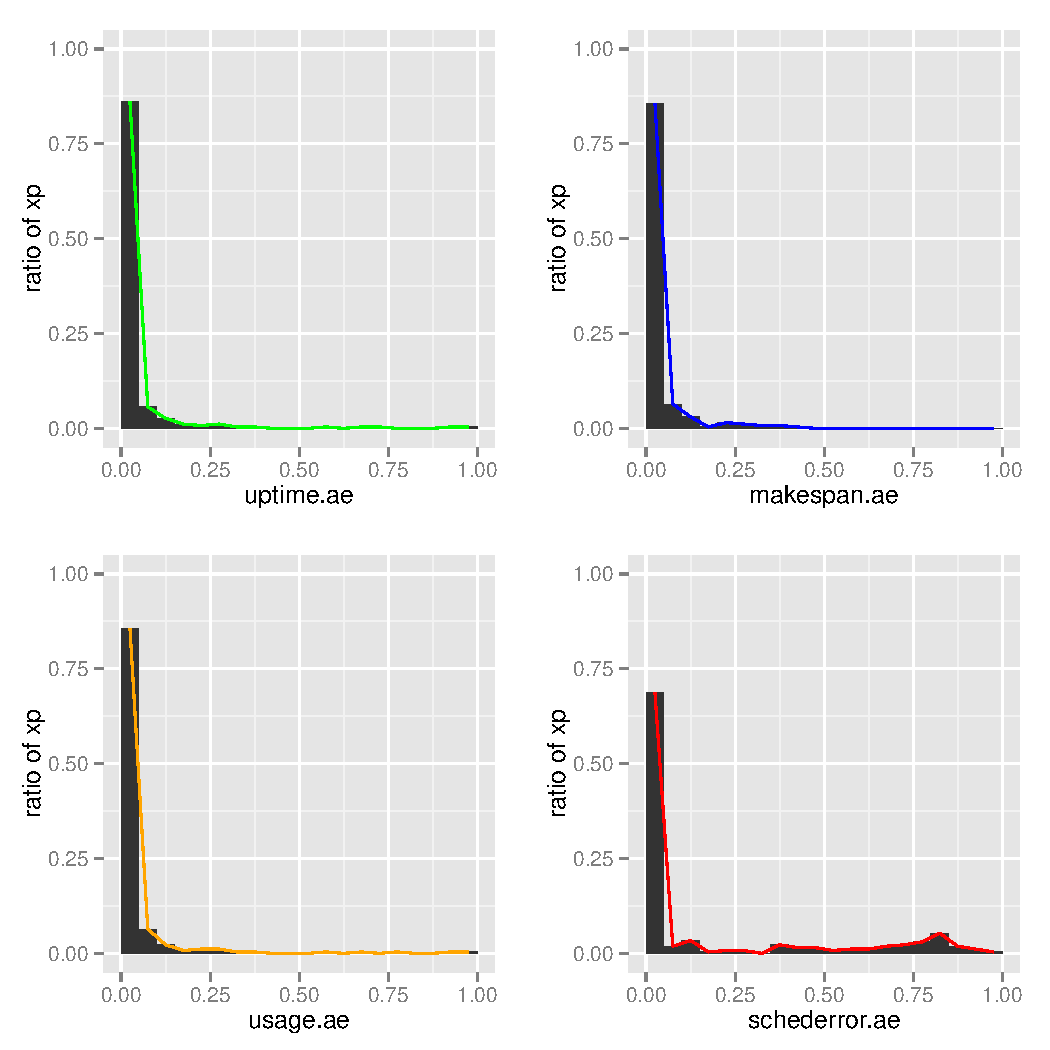
\includegraphics[width=\textwidth]{sim_best-4metrics.pdf}
  
  \input{\vrpath sim_best-4metrics-mmmm.latex}
  
\caption{Frequencies and statistics about absolute error of best simulations (274 xp)}
\end{figure} 

 


% see schiass/lab/setup/simschlouder/validation-results/best-4metrics.dat
\begin{itemize}
 \item uptime: 
      86\% show less than $0.05$ of absolute error, 
      92\% less than $0.10$, 
      2 simulations exceed $0.30$,
      ranging from $0.00$ to $0.50$, for a mean of $0.025$ and a median of $0.001$
 \item makespan: 
      76\% show less than $0.05$ of absolute error, 
      90\% less than $0.10$, 
      0 simulations exceed $0.30$,
      ranging from $0.00$ to $0.62$, for a mean of $0.042$ and a median of $0.018$
 \item usage: 
      59\% show less than $0.05$ of absolute error, 
      91\% less than $0.10$, 
      2 simulations exceed $0.30$,
      ranging from $0.00$ to $0.60$, for a mean of $0.043$ and a median of $0.002$
 \item schederror: 
      70\% show less than $0.05$ of absolute error, 
      72\% less than $0.10$, 
      59 simulations exceed $0.30$,
      ranging from $0.00$ to $0.965$, for a mean of $0.155$ and a median of $0.000$
\end{itemize}

If global metrics are quite accurately assessed by the simulator, 
the scheduling decisions can be very different between simulation and reality. 
One part of the explanation is that scheduling decisions are interdependent: 
any error leads to several others.


\subsection{Simulator accuracy according to platforms and applications}


\begin{figure}
  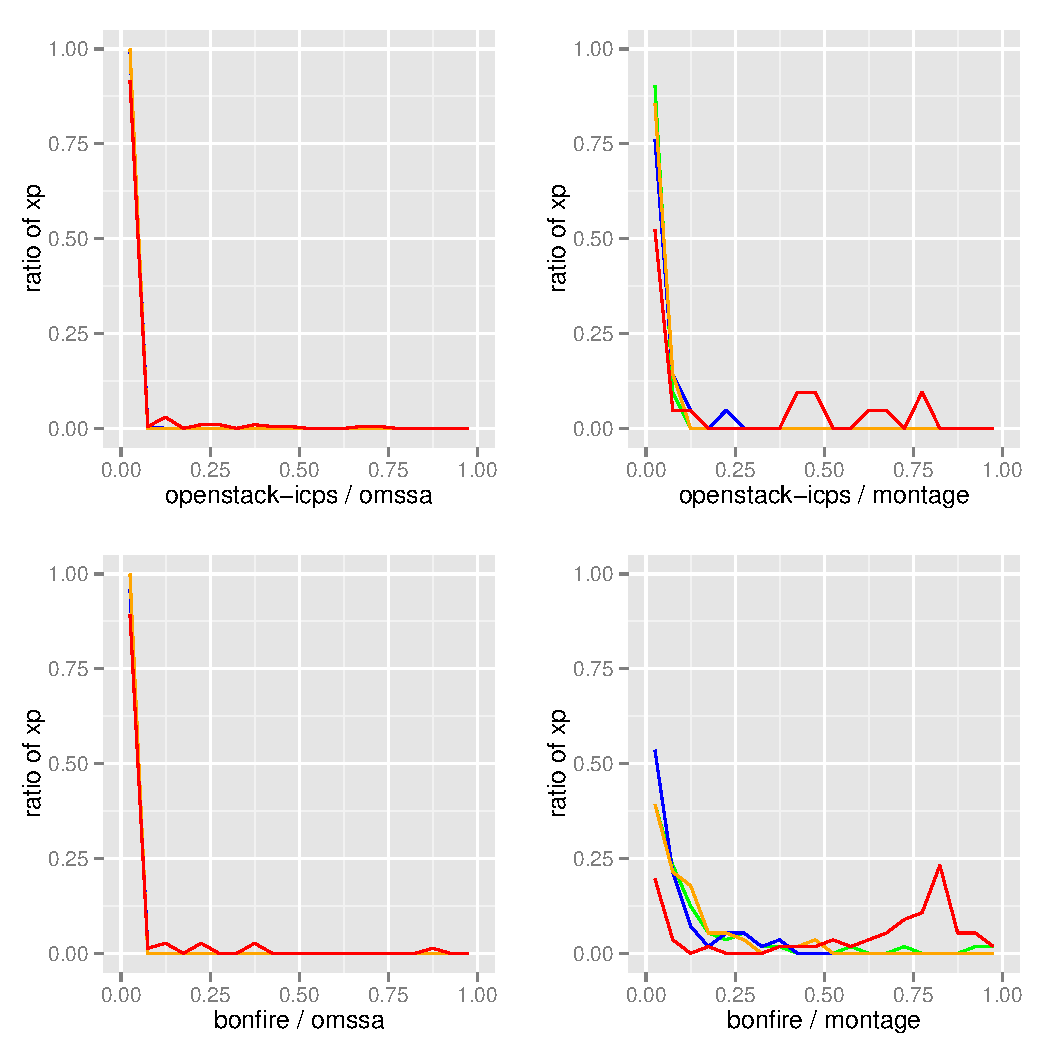
\includegraphics[width=\textwidth]{sim_best-4metrics-platform-app.pdf}
\caption{Absolute error frequencies of best simulations according to platforms 
and applications}
\end{figure} 

\begin{itemize}
 \item openstack-icps / omssa (107 xp): 
 
      \input{\vrpath sim_best-openstack-icps-omssa-4metrics-mmmm.latex}
 
      All metrics are almost perfectly assessed (mean AR from $0.001$ to $0.002$)
      except scheduling error 
      (mean $0.04$ and max $0.75$, 13\% of xp show at least one error), 
      leading to small makespan and usage errors. 
      
      We looked at each single case of scheduling error and all those errors 
      comes from ambiguities in the scheduling algorithms.
      
      This is a first limitation of simulation:
      Whenever heuristics lead to several equivalent solutions, 
      the decision is made by the implementation and relies on data structures 
      (e.g. selection of the first encountered suitable solution) or clocks 
      (e.g. the solution differs from a second to the next, which depends 
      on threads activations and timers). While we made sure to use the same 
      structures and timers, some clocks-related events can not be captured nor 
      simulated: Processing the nodes and tasks queues for scheduling and 
      provisioning decisions take time. Consequently, if those decisions rely on
      clock, they change during the decision process in reality, as clocks advance 
      by itself, but not in simulation, as clocks advance only explicitly.
      
      Thus, the simulation is not mistaken, but only different from reality.
      Actually, the decisions made by the simulator are exactly those that one 
      can expect, while the decisions made by the real scheduler are sometimes
      difficult to understand.

      
\begin{figure}  
  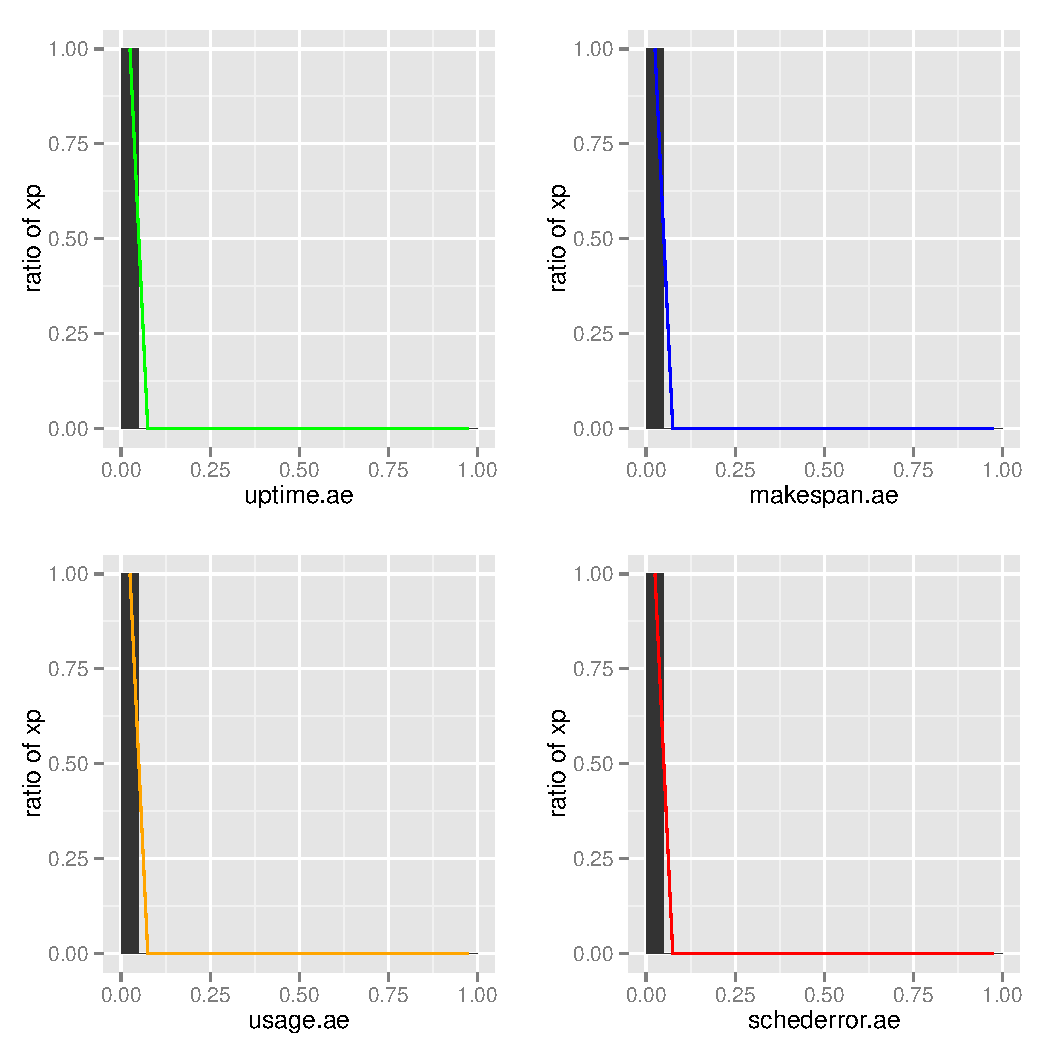
\includegraphics[width=\textwidth]{sim_best-openstack-icps-omssa-noschederror-4metrics.pdf}

  \input{\vrpath sim_best-openstack-icps-omssa-noschederror-4metrics-mmmm.latex}
      
  \input{\vrpath sim_best-openstack-icps-omssa-noschederror-4metrics-mmmm-cmp.latex}

\caption{Frequencies and statistics about absolute error of best simulations for openstack-icps / 
ommssa, without scheduling error cases (91 xps)}
\end{figure}       

      Filtering the xps showing clocks-related issues (16 xps), the results are perfect:
      all metrics present a mean AR of $0.001$, and a max of $0.003$ for uptimes, 
      $0.011$ for makespan, and $0.002$ for usage.
      
      The less accurate simulation actually shows a makespan of 381s instead of 380s
      as in the real xp. This is due to an imperfection of our simulator:
      While task management latencies are included into the walltimes in real traces,
      they come in addition of this walltimes in the simulator.
      This is a problem only when comparing simulations to real traces, but allows
      regular usage of the simulator to assess task management latencies.

      This shows that, providing that one can inject the right information, 
      the only limitation of our simulator are micro clock-related hazards.
      
      
 \item openstack-icps / montage (36 xps): 
 
      \input{\vrpath sim_best-openstack-icps-montage-4metrics-mmmm.latex}

      \input{\vrpath sim_best-openstack-icps-montage-4metrics-mmmm-cmp.latex}

      With a work-flow, scheduling errors are more numerous 
      (AR mean of $0.24$ for a max of $0.79$), leading to less accurate assessments
      of uptime, makespan and usage (mean AR of $0.01$, $0.05$, and $0.01$), that
      is ten times more than with a BoT.
      
      First, montage has much more tasks (from 43 to 1672) than omssa (from 33 to 223).
      Consequently, queues are much longer, which increases the clock-related issues.
      
      BoT scheduling are actually made offline (i.e. scheduling decisions are taken
      before any actual execution), while WF scheduling implies decisions during 
      the execution, every time dependencies are satisfied. 
      Those decisions rely on the system state (predicted end date of nodes for 
      instance). Consequently, divergences between simulation and reality have
      more important impacts.
      
      %Worst case: v3.standard.2x2.asap.regular.openstack-icps.1 
      %first proverror: 2mass_pleiades_2x2_gather
      %Log of schlouder shows that all solutions are elligible, 
      %but it shouldn't be this one (which is in the middle of the queue)... Mystery!
      
      For instance, the worst case shows a very large amount of scheduling errors 
      (0.954). A close examination of this case shown that the simulation behave
      as expected : After the first dependencies were satisfied,
      three newly ready tasks $t1$, $t2$, and $t3$ were scheduled on the node $n$.
      However in reality, scheduling takes time. During this time, the last task
      scheduled to node $n$ was completed between the scheduling of $t2$ and $t3$, 
      but before $t1$ were actually submitted to $n$. This lead to mistakingly 
      set the state of node $n$ to idle, impacting the scheduling decision of $t3$.
      
      Those kind of complex and unforeseeable events are actually frequent 
      when confronted to reality. However, they are utterly difficult to detect
      (1672 jobs were scheduled for the presented case).
      Comparing real execution with simulation allow the detection of such case, 
      without having to look at each scheduling decision.
      
      the last task assigned to node $n$ was 
      completed during the scheduling of the tasks which dependencies were satisfied 
      first. But those tasks were intended to 
      This completion lead 
      Schlouder to mistake the state of the 
      
      
 
 \item bonfire / omssa (75 xp): 
 
      \input{\vrpath sim_best-bonfire-omssa-4metrics-mmmm.latex}
      
      \input{\vrpath sim_best-bonfire-omssa-4metrics-mmmm-cmp.latex}
      
      On a public shared heterogeneous cloud, scheduling errors are more numerous 
      (AR mean of $0.03$ for a max of $0.86$), leading to less accurate assessments
      of uptime, makespan and usage (mean AR of $0.005$, $0.045$, and $0.053$).

      More interesting, usage are never perfectly assessed: 
      16\% of xp show less than $0.05$ of AR, 
      while 86\% show an AR between $0.05$ and $0.10$
      
      This show the impacts of public heterogeneous platforms on simulation
      accuracy: 
      It is not possible to precisely simulate the vm-to-pm scheduling algorithm of 
      public cloud, as they are generally not public, and their decisions impacts 
      performances, as one can not predict the power of the VM one get.
 
 \item bonfire / montage (56 xp): 
 
      \input{\vrpath sim_best-bonfire-montage-4metrics-mmmm.latex}
      
      \input{\vrpath sim_best-bonfire-omssa-4metrics-mmmm-cmp.latex}
 
      On a public shared heterogeneous cloud, scheduling errors are even more numerous 
      (AR mean of $0.48$ for a max of $0.96$), leading to less accurate assessments
      of uptime, makespan and usage (mean AR of $0.10$, $0.115$, and $0.48$).
      
      This is simply explained by the cumulation of inaccuracies from 
      both platform and applications. 
\end{itemize}



\subsection{Boottime impacts}

Assessing the impact of efficient boottimes simulation.

Same simulations, without injecting the boottimes observations. 
Thus, boottimes are only predictions, based on linear regressions of previously
observed boottimes.

\begin{figure}
  \centering
  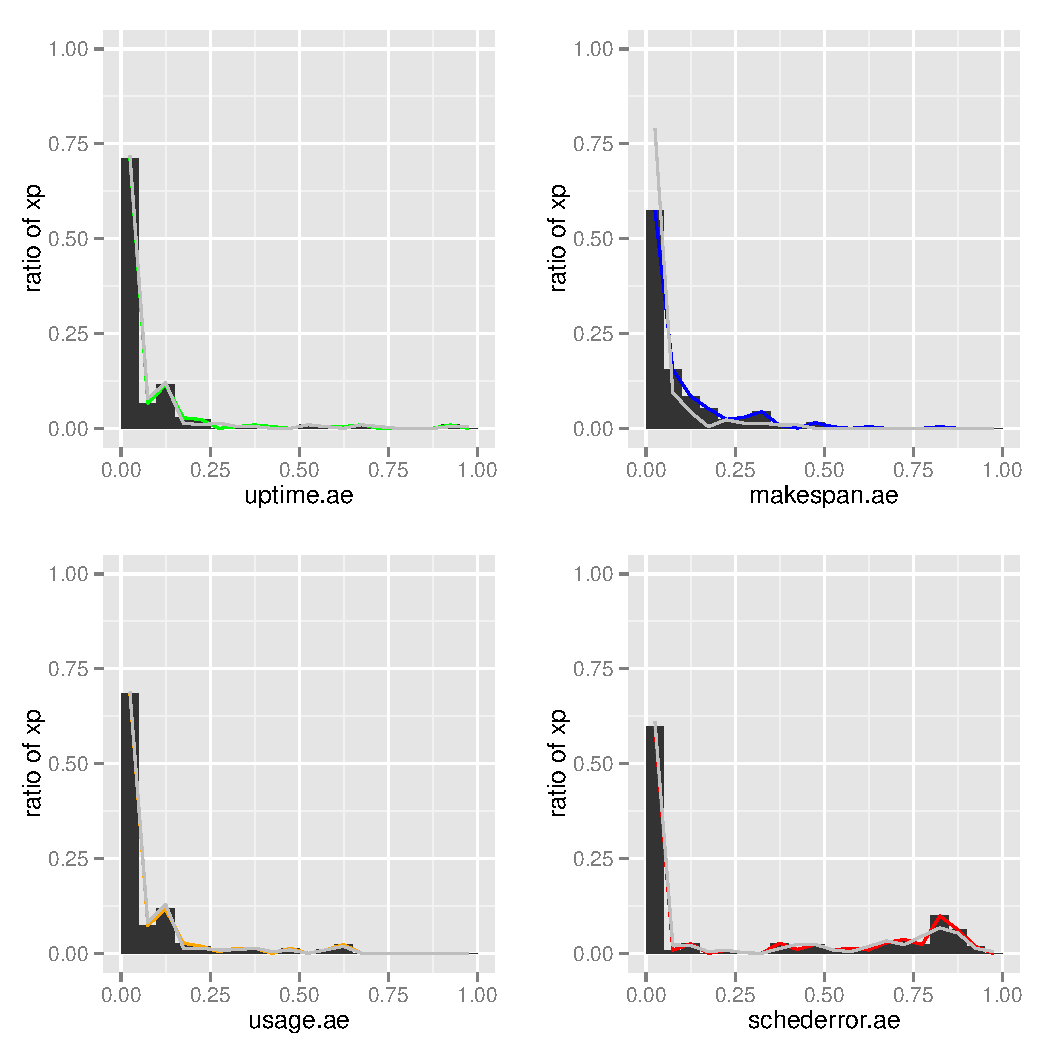
\includegraphics[width=\textwidth]{sim_no-boottimes-4metrics-cmp.pdf}

  \input{\vrpath sim_no-boottimes-4metrics-mmmm.latex}

  \input{\vrpath sim_no-boottimes-4metrics-mmmm-cmp.latex}

  \input{\vrpath sim_no-boottimes-4metrics-mmmm-twobytwo.latex}

  \caption{Frequencies, statistics, and comparison with best of simulations with no real boot times 
  injection}

\end{figure} 

%worst case: v3.standard.2x2.asap.regular.fr-inria.2 
The worst case show a makespan ae of $0.816$ (3141s instead of 17076s). 
This is due to boottimes on BonFire that were completely of charts: 
5 boots were normal (ranging from 232s to 311s), 
the 17 others ranged from 3281s to 11084s.
Whereas BonFire were intended to deliver 22 simultaneous VMs, only 5 were available
at the time of the experiment. Instead of refusing the following 17 VMs, the
provisioning system of BonFire put them in pending state, waiting for the delivered
ones to stop. The VMs being provisioned for one hour, following the 5 normal boots, 
5 boots took approximatively 1 hour, then 5 other boots took 2 hours,
and 5 another more took 3 hours. Finally, 2 boots took 1 hour after the last 
dependencies were satsified.

This illustrates that defective clouds can not be efficiently simulated without 
proper information capture. However, once captured, this kind of defection is
perfectly simulated by SchIaaS. Consequently, it can be used to assess behavior 
and robustness of solutions facing these defections.

%Best case: v3.standard.3x3.afap.regular.de-hlrs.2
Some case are surprisingly improved without the real boot times injection:
For instance, one xp shows a real makespan of 25788s, for 35106s with boot times
injection and 24266s without. 




\subsubsection{No-threads}

Injection of: real boot times and some times due to Schlouder internal threads, 
such as lapses after a node become ready and the start of the first job.

Assess the impact of efficient internal threads simulation

\begin{figure}
  \centering
  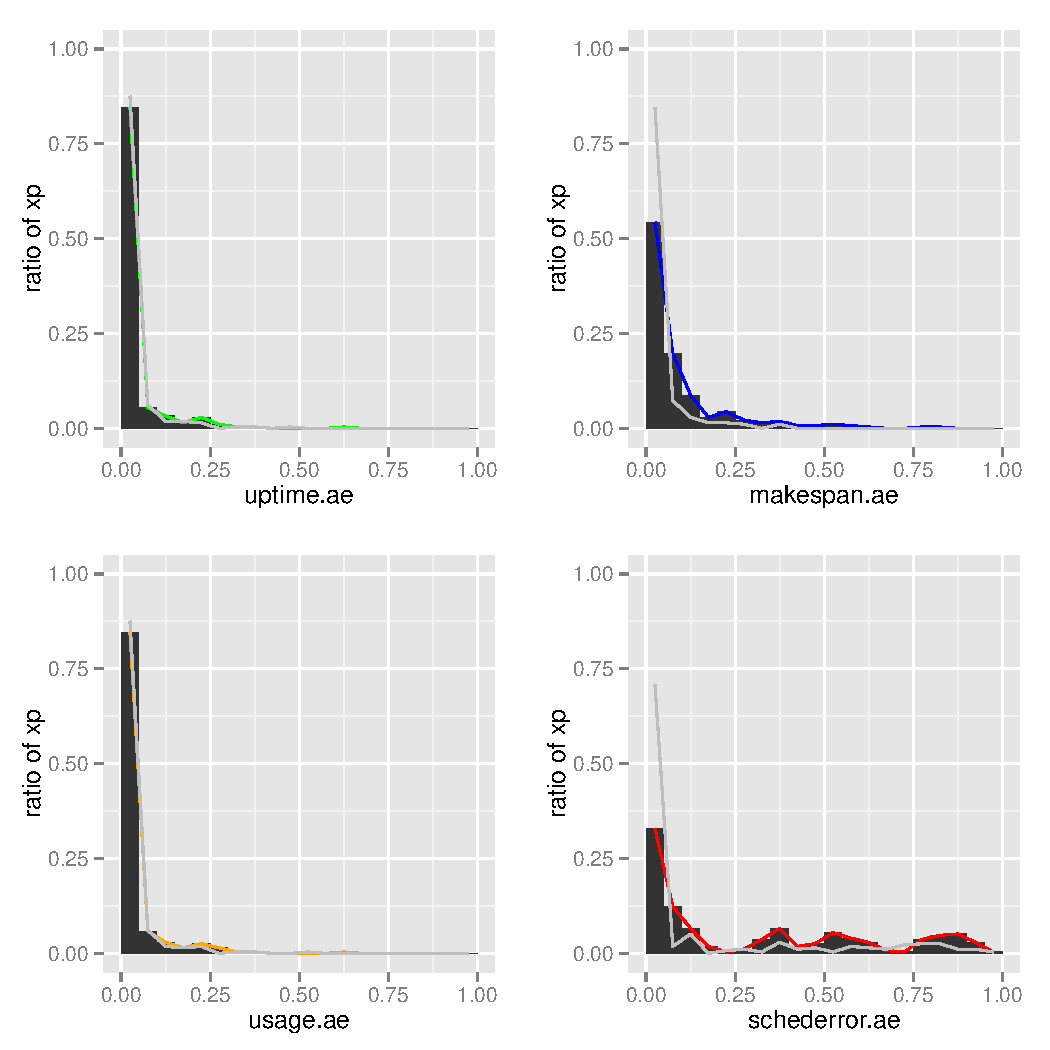
\includegraphics[width=\textwidth]{sim_no-threads-4metrics-cmp.pdf}
  
  \input{\vrpath sim_no-threads-4metrics-mmmm.latex}

  \input{\vrpath sim_no-threads-4metrics-mmmm-cmp.latex}

  \input{\vrpath sim_no-threads-4metrics-mmmm-twobytwo.latex}
    
  \caption{Frequencies, statistics, and comparison with best of simulations with no real thread times
  injection}
\end{figure} 



\subsubsection{Communications}

Injection of: real boot times, some times due to Schlouder internal threads, 
such as lapses after a node become ready and the start of the first job, 
and, real runtimes and real data size for jobs input and output communications.

Assess the impact of efficient communications 

\begin{figure}
  \centering
  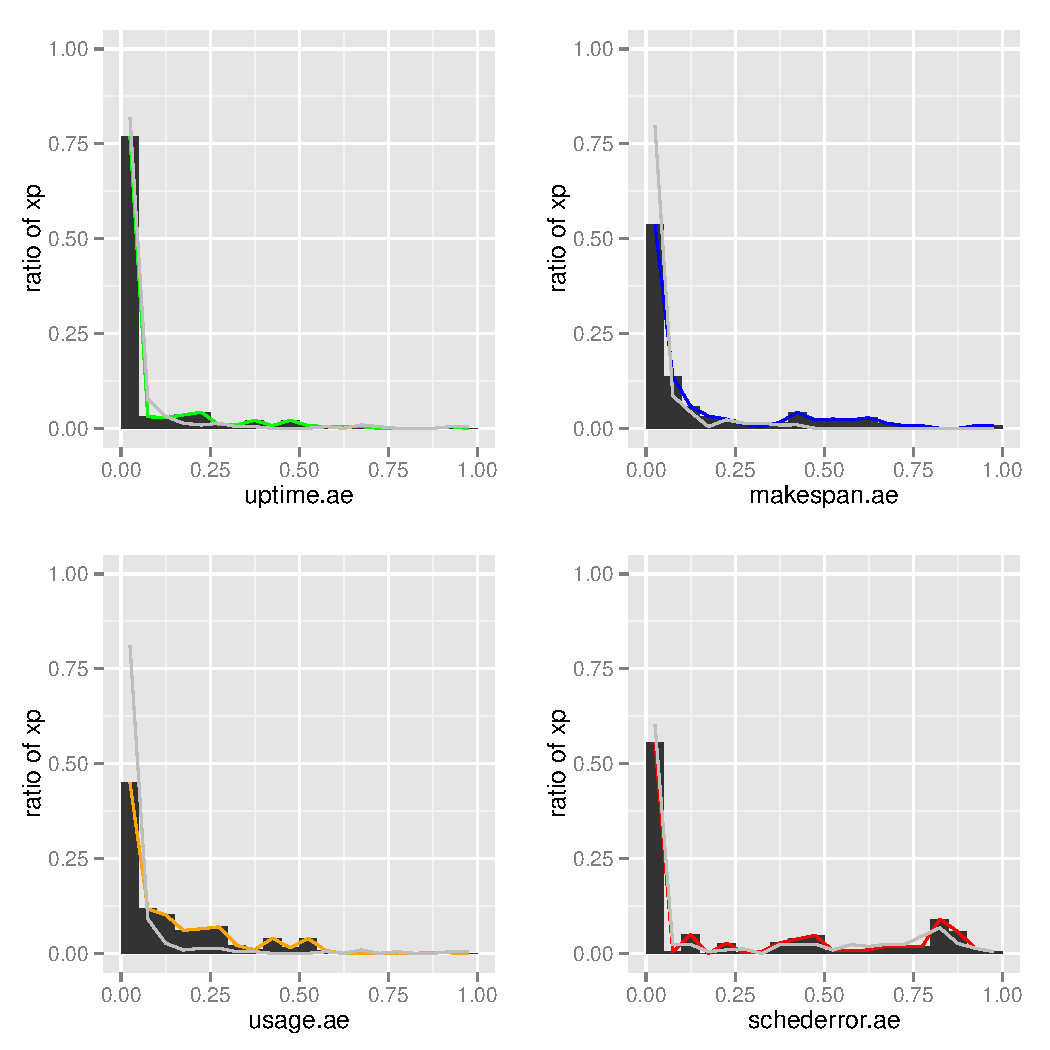
\includegraphics[width=\textwidth]{sim_communications-4metrics-cmp.pdf}
  
  \input{\vrpath sim_communications-4metrics-mmmm.latex}

  \input{\vrpath sim_communications-4metrics-mmmm-cmp.latex}

  \input{\vrpath sim_communications-4metrics-mmmm-twobytwo.latex}

  \caption{Frequencies, statistics, and comparison with best of simulations with simulation of communications}
\end{figure} 

\begin{figure}
  \centering
  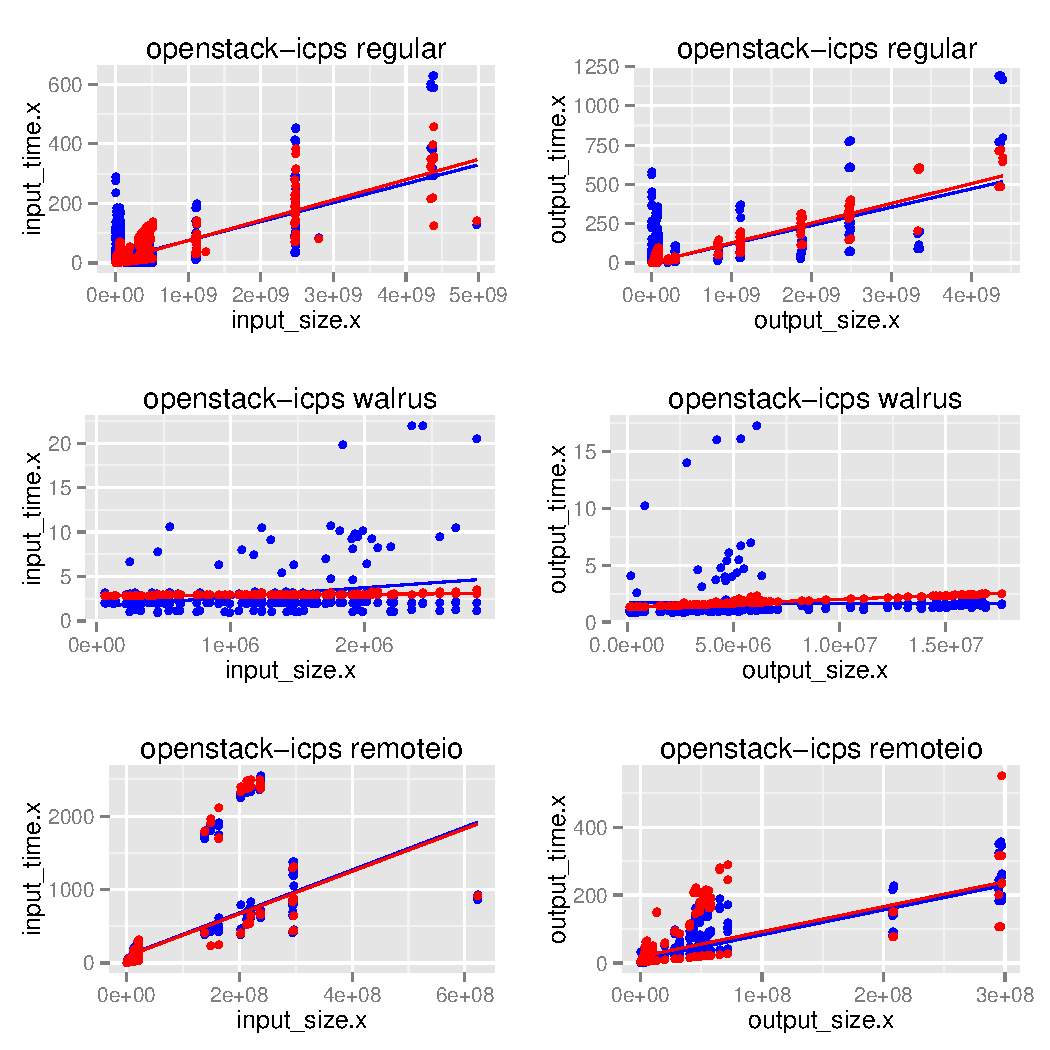
\includegraphics[width=\textwidth]{communications-openstack-icps.pdf}
  
  \caption{Linear regressions of communication times vs. data size, 
    according to platform, storage, and communication direction on openstack-icps}
\end{figure} 


\begin{figure}
  \centering
  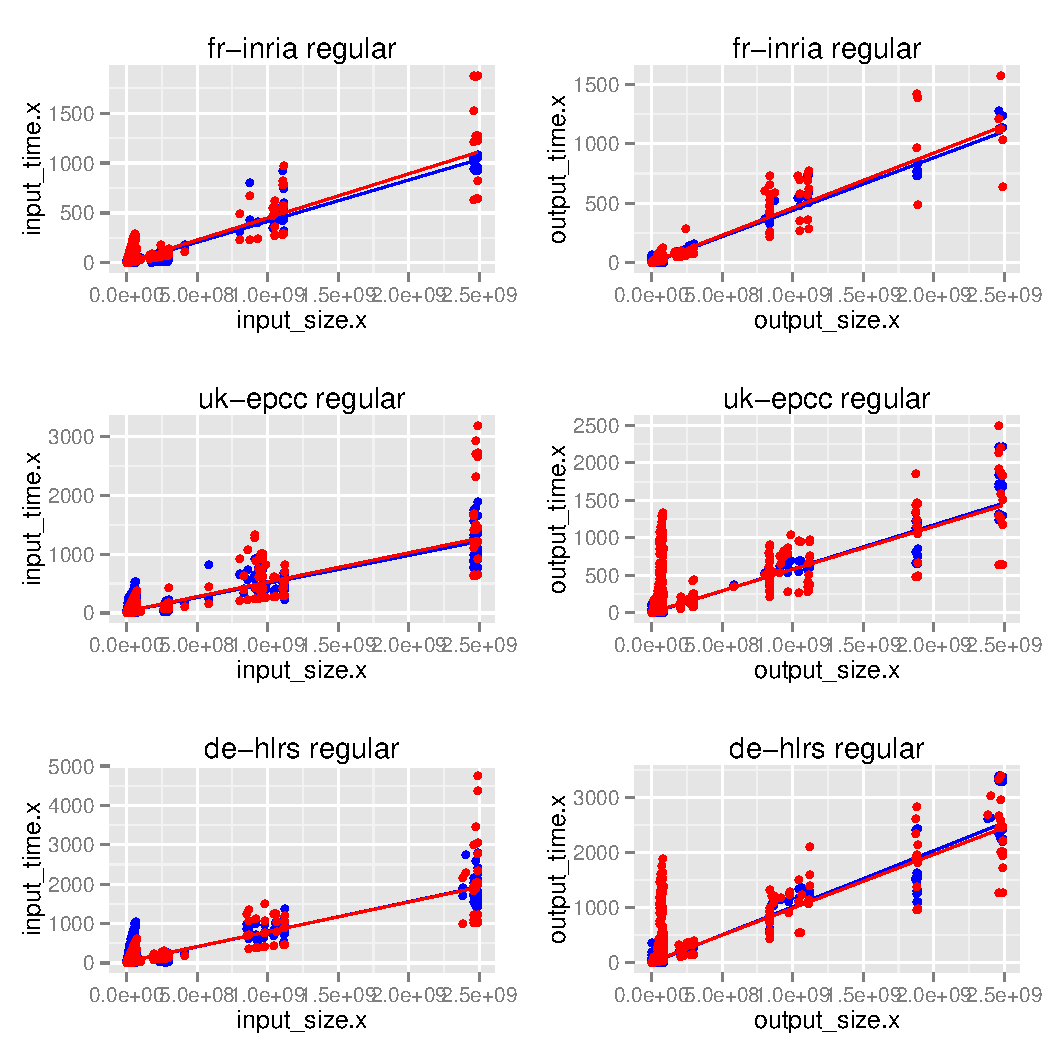
\includegraphics[width=\textwidth]{communications-bonfire.pdf}
  
  \caption{Linear regressions of communication times vs. data size, 
    according to platform, storage, and communication direction on BonFire}
\end{figure} 


\subsubsection{Prediction}

Injection of nothing from the real xp, except the xp description as submitted 
to schlouder.

Assess the efficiency of using a simulator as a predictor of a cloud.

\begin{figure}
  \centering
  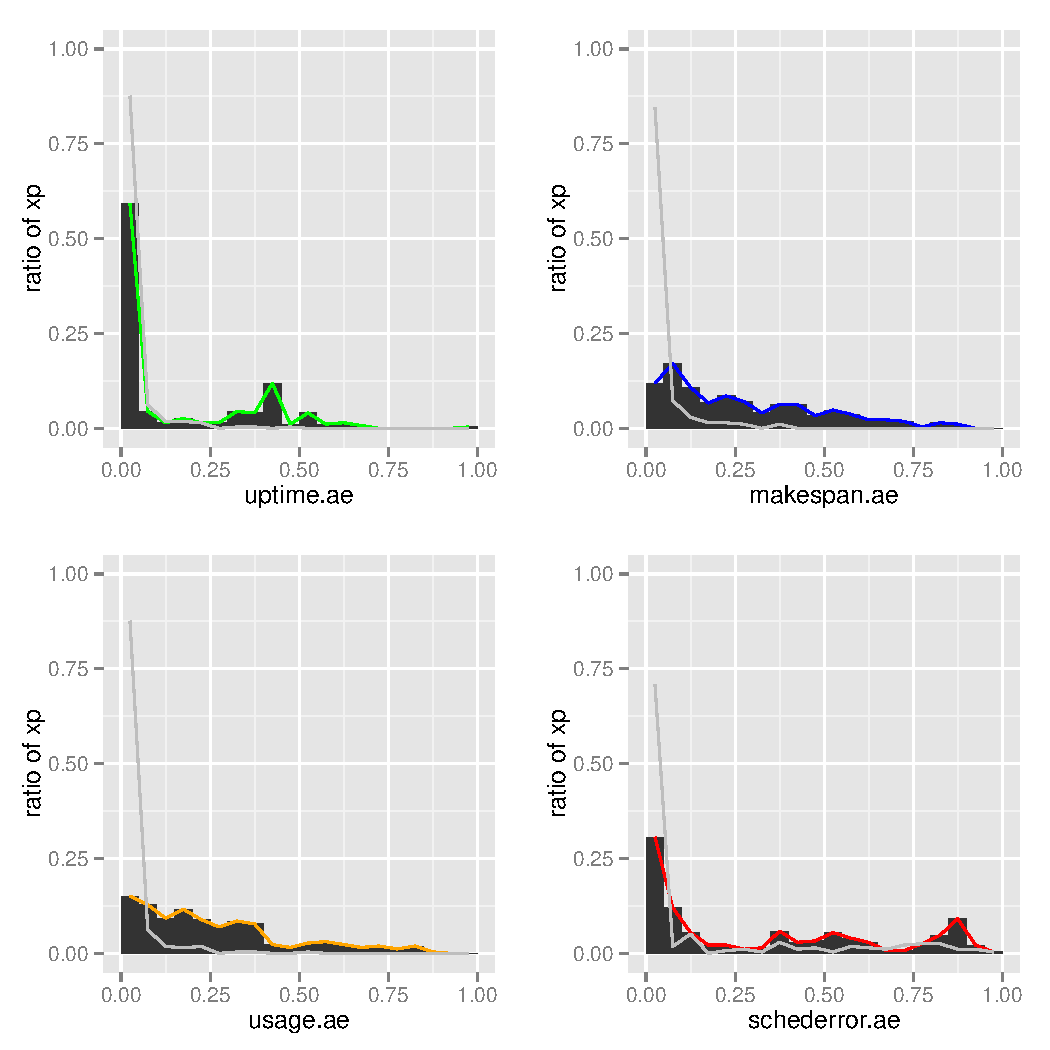
\includegraphics[width=\textwidth]{sim_predictions-4metrics-cmp.pdf}
  
  \input{\vrpath sim_predictions-4metrics-mmmm.latex}

  \input{\vrpath sim_predictions-4metrics-mmmm-cmp.latex}

  \input{\vrpath sim_communications-4metrics-mmmm-twobytwo.latex}

  
  \caption{Frequencies, statistics, and comparison with best of simulations with no injection}
\end{figure} 

\section{Open-science}

\begin{verbatim}
git clone https://git.unistra.fr/gossa/schlouder-traces.git
git clone https://scm.gforge.inria.fr/anonscm/git/schiaas/schiaas.git 
cd schiaas
cmake .
make
cd lab
./lap.py -p2 setup/simschlouder/validation.cfg
cd setup/simschlouder/validation-results
ls
\end{verbatim}

\end{document}


